% =====================================================================
% OPTION A — Academic / CVPR-style
% A0 vertical (841 mm × 1189 mm). Two-column body, navy accents,
% information-dense like a conference poster.
% =====================================================================
\documentclass[a0paper, portrait]{article}

\usepackage[paperwidth=841mm, paperheight=1189mm,
            top=18mm, bottom=18mm, left=25mm, right=25mm]{geometry}
\usepackage[T1]{fontenc}
\usepackage{lmodern}
\usepackage{microtype}
\usepackage{parskip}
\usepackage{amsmath, amssymb}
\usepackage{tikz}
\usetikzlibrary{positioning, shapes.geometric, calc, arrows.meta, fit}
\usepackage{tcolorbox}
\tcbuselibrary{skins}
\usepackage{graphicx}
\usepackage[table]{xcolor}
\usepackage{multicol}
\usepackage{booktabs}
\usepackage{tabularx}
\usepackage{qrcode}
\usepackage{enumitem}

\pagestyle{empty}

% --- palette ---
\definecolor{Navy}{HTML}{1F6FEB}
\definecolor{Dark}{HTML}{1A1A2E}
\definecolor{Light}{HTML}{66667A}
\definecolor{GoodGreen}{HTML}{2CA02C}
\definecolor{BadRed}{HTML}{D62C2E}
\definecolor{LightBlue}{HTML}{F0F6FF}
\definecolor{LightGreen}{HTML}{E8F7E8}
\definecolor{LightRed}{HTML}{FDECEC}
\definecolor{LightGray}{HTML}{F5F5F7}

\graphicspath{
    {../../report/figures/}
    {../../presentation/_build/}
}

% Section heading box
\newtcolorbox{secbox}[1]{%
    colback=LightBlue, colframe=Navy,
    coltitle=white, fonttitle=\bfseries\Huge,
    title={#1},
    arc=4mm, boxrule=0.6mm,
    left=8mm, right=8mm, top=4mm, bottom=4mm,
    fontupper=\Large
}

\setlist[itemize]{leftmargin=*, itemsep=2mm}

\begin{document}
\begin{center}

% =====================================================================
% TITLE BAR
% =====================================================================

\begin{tikzpicture}[remember picture]
\node[rectangle, fill=Navy, minimum width=781mm, minimum height=130mm,
      anchor=north, inner sep=10mm] at (0, 0) {%
    \begin{minipage}{700mm}
        \centering
        {\color{white!85}\bfseries\fontsize{26}{32}\selectfont
        BOCCONI UNIVERSITY \quad$\cdot$\quad COMPUTER VISION \&\ IMAGE PROCESSING}\\[5mm]
        {\color{white}\bfseries\fontsize{82}{92}\selectfont
        Feedback-Augmented RT-DETR}\\[4mm]
        {\color{white!90}\itshape\fontsize{40}{46}\selectfont
        A Cross-Attention Refinement Strategy for Small-Object Detection}\\[6mm]
        {\color{white}\fontsize{32}{38}\selectfont
        Hatem Saadallah\quad$\cdot$\quad Nour Jennane}
    \end{minipage}
};
\end{tikzpicture}

\vspace{12mm}

% =====================================================================
% HEADLINE STRIP — one number that sells the whole poster
% =====================================================================

\begin{tikzpicture}
\node[draw=GoodGreen, line width=2.5mm, fill=LightGreen,
      rounded corners=8mm, inner sep=10mm,
      minimum width=700mm] {%
    \begin{minipage}{650mm}
        \centering
        {\fontsize{32}{38}\selectfont\color{Dark}Causal contribution
        of feedback on COCO val2017:}\\[3mm]
        {\fontsize{160}{160}\selectfont\bfseries\color{GoodGreen}+0.99}\\[1mm]
        {\fontsize{32}{38}\selectfont\color{Dark}small-object AP \quad
        \textcolor{Light}{(33.26 \;$\to$\; 34.25, same checkpoint, ON $-$ OFF)}}
    \end{minipage}
};
\end{tikzpicture}

\vspace{10mm}

% =====================================================================
% BODY — two columns
% =====================================================================
\begin{minipage}[t]{0.485\textwidth}

\begin{secbox}{1.\quad The Problem}
RT-DETR achieves real-time, NMS-free object detection. Yet on COCO
\textsc{val2017}, RT-DETR-R50 reports
{\bfseries\color{BadRed}AP\textsubscript{S}\,=\,34.7} for small objects
versus {\bfseries\color{GoodGreen}AP\textsubscript{L}\,=\,67.7} for large
ones --- a 33-point gap on the same network.

\medskip
\textbf{Why?} Encoder memory is computed once before any decoder layer
fires. As the decoder discovers object hypotheses, that information
cannot flow back to revise the features it is reading from. Refinement
is strictly one-way.
\end{secbox}

\bigskip

\begin{secbox}{2.\quad Our Idea}
\begin{center}

\includegraphics[width=0.85\linewidth]{diag_idea.png}
\end{center}
\medskip
After the first decoder layer makes preliminary predictions, use them
as keys/values in a single cross-attention pass that refines the
encoder memory. Layers $2{-}L$ then attend over the refined memory:
\[
\boxed{\;
\mathbf{m}' \;=\; \mathbf{m} \;+\; g \cdot
\mathrm{Attn}(\mathbf{m},\, \mathbf{t}^{(1)})
\;}
\]
where $g \in (0,1)$ is a learnable scalar gate.
\end{secbox}

\bigskip

\begin{secbox}{3.\quad v1: Trained but Silent}
We added the module with a plain sigmoid gate
($g = \sigma(\alpha)$, $\alpha_{\mathrm{init}} = -2$) applied to all four
pyramid levels. Training was clean. The same-checkpoint inference
ablation gave:
\begin{center}
\fontsize{72}{72}\selectfont\bfseries\color{BadRed}
$\Delta$AP\textsubscript{S} = 0.00
\end{center}
The gate had decayed to ${\approx}\,0.12$ during training. The
cross-attention output was multiplied by ${\approx}\,0$ before reaching
memory --- statistically identical to skipping the module.
\end{secbox}

\bigskip

\begin{secbox}{4.\quad v2: Two Structural Fixes (Zero New Params)}
\begin{itemize}
    \item \textbf{Gate floor reparameterization.}\\
          $g_{\mathrm{eff}} = \mathrm{floor} + (1-\mathrm{floor})\cdot\sigma(\alpha),
          \;\; \mathrm{floor}=0.1$.\\
          The optimizer can attenuate, never silence.
    \item \textbf{Level mask: P2/P3 only.}\\
          Refine the stride-4 and stride-8 features (where small objects
          live); leave P4, P5 untouched.
\end{itemize}

\medskip
\begin{center}
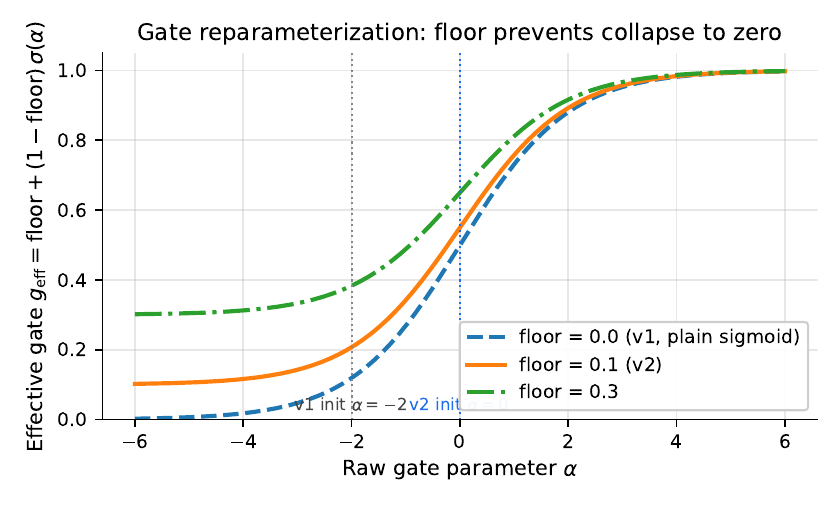
\includegraphics[width=0.92\linewidth]{gate_reparam.png}
\end{center}
\end{secbox}

\end{minipage}
\hfill
\begin{minipage}[t]{0.485\textwidth}

\begin{secbox}{5.\quad Same-Checkpoint Ablation}
\begin{center}
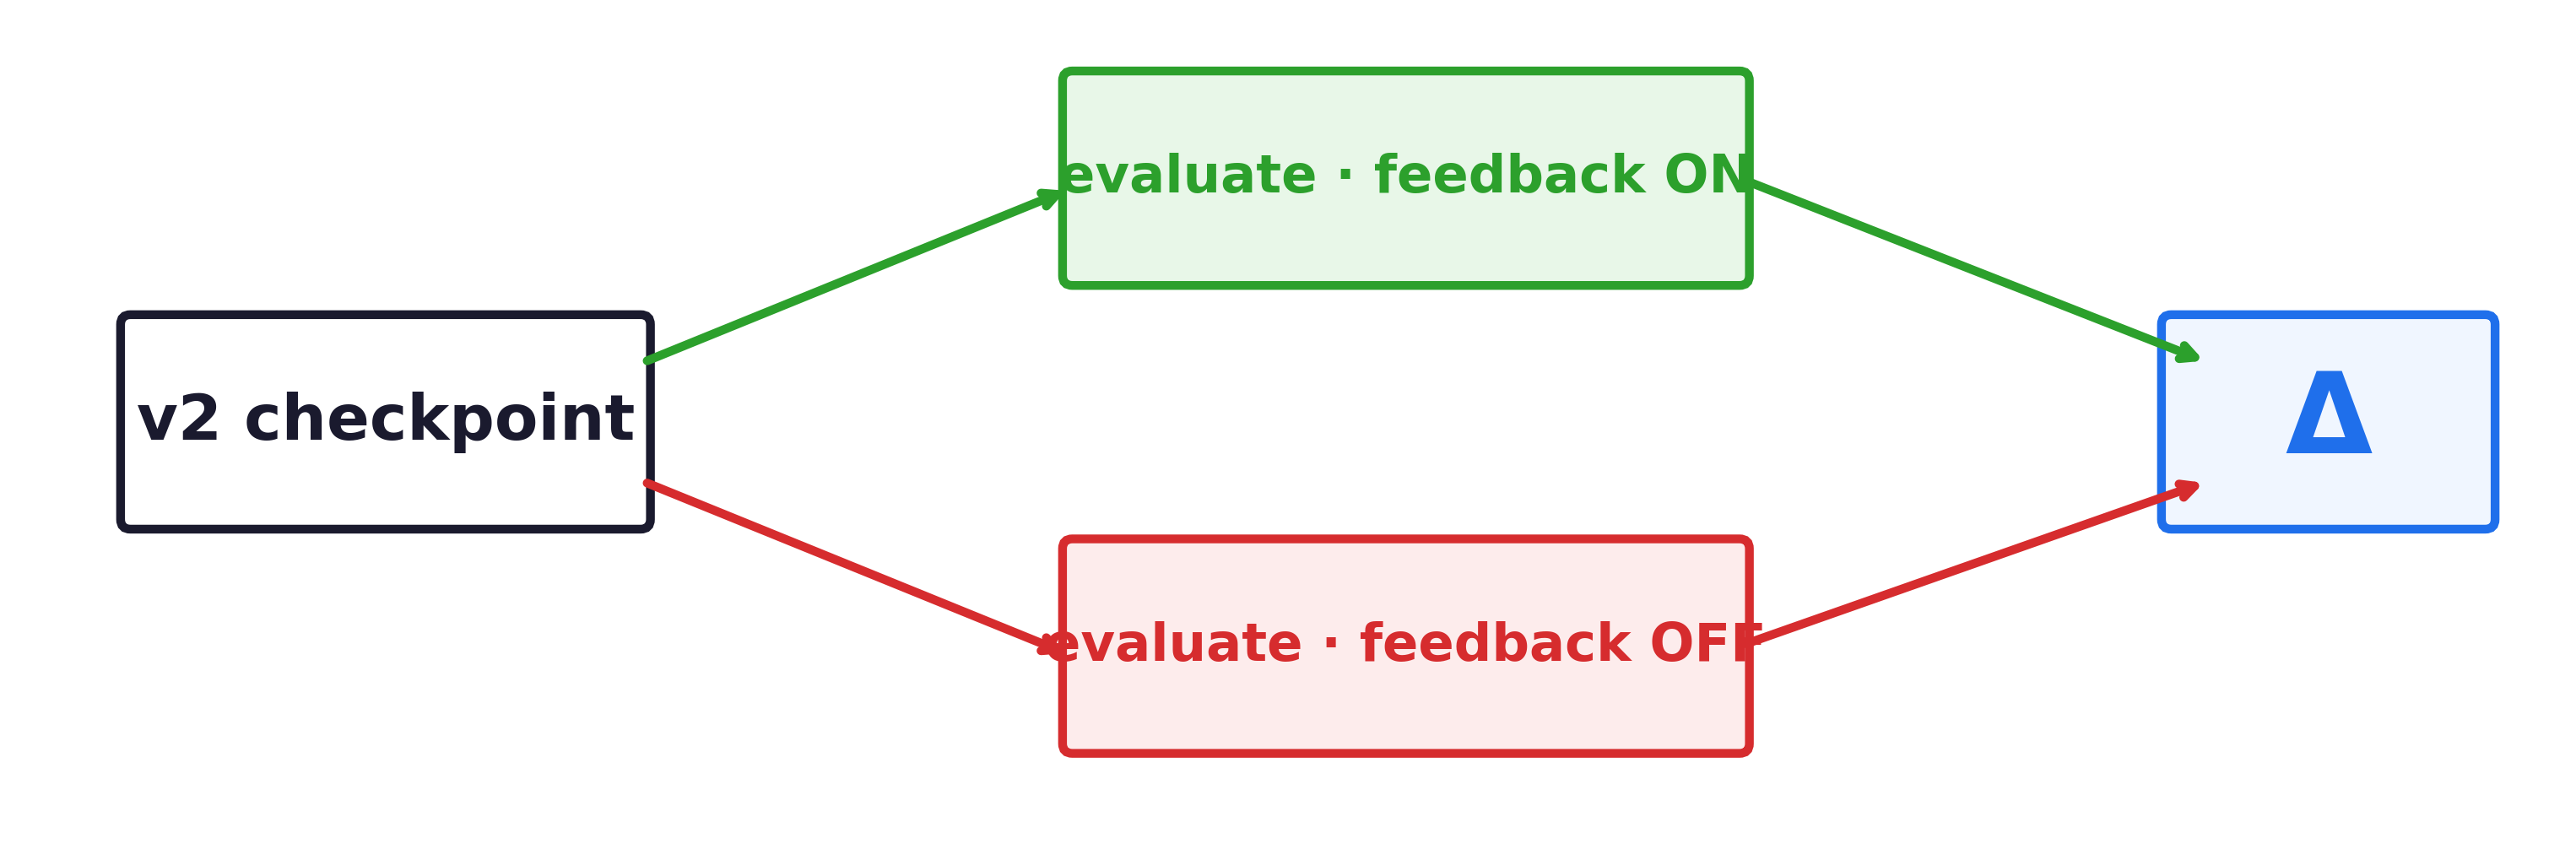
\includegraphics[width=0.95\linewidth]{diag_ablation.png}
\end{center}

\medskip
Two evaluations of identical weights, identical inputs --- the only
difference is whether the feedback module's forward call fires at
inference. Any difference in metrics is therefore attributable to the
feedback computation alone.
\end{secbox}

\bigskip

\begin{secbox}{6.\quad Results}
\begin{center}
\renewcommand{\arraystretch}{1.4}
\begin{tabularx}{\linewidth}{lccccc}
    \toprule
    \textbf{Model} & \textbf{Mode} & \textbf{AP} &
    \textbf{AP\textsubscript{S}} & \textbf{AP\textsubscript{M}} &
    \textbf{AP\textsubscript{L}} \\
    \midrule
    Feedback v1 & ON  & 52.01 & 33.91 & 56.28 & 68.83 \\
    Feedback v1 & OFF & 51.92 & 33.91 & 56.18 & 68.63 \\
    \rowcolor{LightGray}
    \textbf{v1 $\Delta$ causal}  & --- & $+0.09$ &
    \textcolor{BadRed}{\textbf{0.00}} & $+0.10$ & $+0.20$ \\
    \midrule
    Feedback v2 & ON  & 52.10 & \textbf{34.25} & 56.33 & 68.82 \\
    Feedback v2 & OFF & 51.53 & 33.26 & 55.91 & 68.32 \\
    \rowcolor{LightGreen}
    \textbf{v2 $\Delta$ causal}  & --- & $+0.57$ &
    \textcolor{GoodGreen}{\textbf{+0.99}} & $+0.42$ & $+0.50$ \\
    \bottomrule
\end{tabularx}
\end{center}

\medskip
\begin{center}
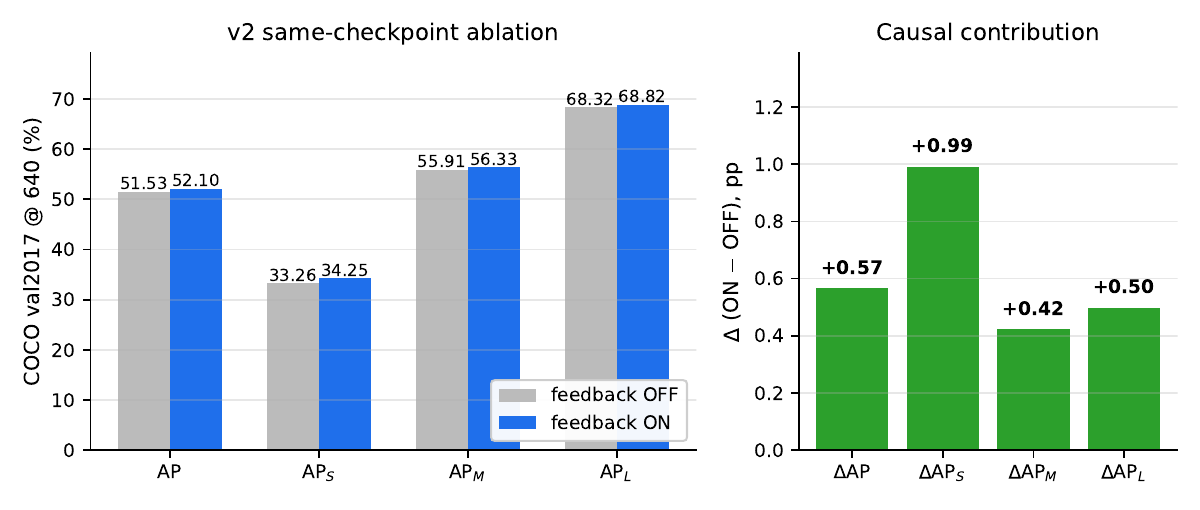
\includegraphics[width=\linewidth]{ablation_bars.png}
\end{center}
\end{secbox}

\bigskip

\begin{secbox}{7.\quad Training Trajectory}
\begin{center}
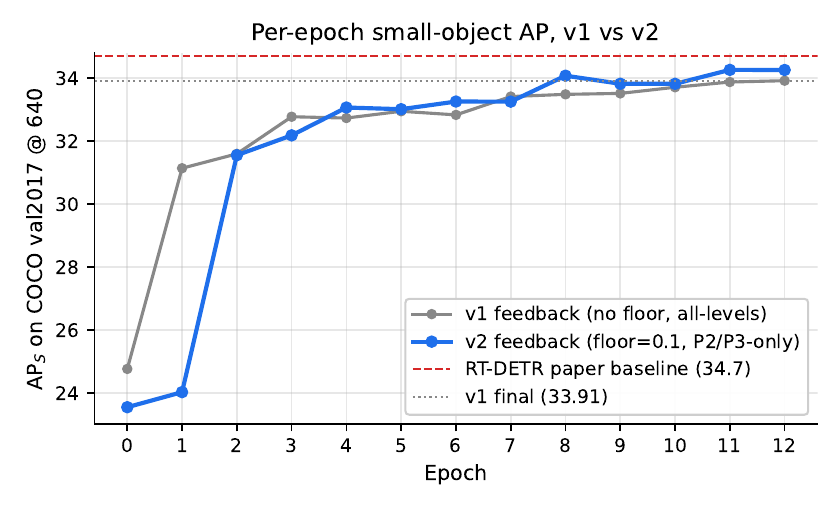
\includegraphics[width=0.92\linewidth]{learning_curves.png}
\end{center}
v2 first crosses v1's eventual final $33.91$ at \textbf{epoch 8} ---
four epochs early.
\end{secbox}

\bigskip

\begin{secbox}{8.\quad Limitations \& Future Work}
\textbf{Limitations.}
\begin{itemize}\setlength\itemsep{0.5mm}
    \item Single seed; multi-seed variance unmeasured.
    \item 13-epoch finetune (vs 72-epoch from scratch).
    \item Floor and mask not isolated --- a $2{\times}2$ ablation
          would resolve.
    \item ${\approx}\,2{\times}$ slower (cost is the P2 level, not feedback).
\end{itemize}

\medskip
\textbf{Future work --- recovering FPS.}
\begin{itemize}\setlength\itemsep{0.5mm}
    \item \emph{Train with P2, infer without.}\\
          {\color{Light}\small Keep the gain; recover ${\approx}\,53$ FPS.}
    \item \emph{Lighter P2 path} (fewer channels / simpler projection).
    \item \emph{Knowledge distillation} v2\,$\to$\,P3--P5 student.
\end{itemize}
\end{secbox}

\end{minipage}

\vspace{8mm}

% =====================================================================
% FOOTER — combined takeaway + repo + QR in one compact band
% =====================================================================

\begin{tikzpicture}
\node[rectangle, fill=Dark, minimum width=791mm, minimum height=130mm,
      anchor=north, inner sep=10mm] {%
    \begin{minipage}{770mm}
        \begin{minipage}[c]{555mm}
            \raggedright\color{white}
            {\fontsize{32}{38}\selectfont\bfseries
            \emph{An unconstrained sigmoid gate lets the optimizer
            silence a new mechanism --- a floor closes that route.}}\\[4mm]
            {\color{white!80}\fontsize{24}{30}\selectfont
            The difference between a null and a +0.99 ablation. \;
            Built on RT-DETR (Lyu et al., CVPR 2024).}\\[3mm]
            {\fontsize{22}{26}\selectfont\bfseries\color{Navy!50!white}
            github.com/HatemSaadallah/feedback-augmented-rtdetr}
        \end{minipage}\hfill
        \begin{minipage}[c]{170mm}
            \centering
            \fcolorbox{white}{white}{\qrset{height=80mm}\qrcode{https://github.com/HatemSaadallah/feedback-augmented-rtdetr}}\\[2mm]
            {\fontsize{20}{24}\selectfont\color{white!70}scan for code \&\ paper}
        \end{minipage}
    \end{minipage}
};
\end{tikzpicture}

\end{center}
\end{document}
